\section{Methodology: LoRA Subspace Projection Routing}
\label{sec:method}

We present \textbf{LoRA Subspace Projection Routing (LSPR)}, a joint training-and-routing paradigm that achieves dynamic model ensembling by exploiting the intrinsic linear-algebraic structure of Low-Rank Adaptation (LoRA) weights. While the online routing mechanism itself is training-free, requires zero task-specific calibration data, and is completely classification-head-free at deployment time, LSPR requires that individual adapters be trained using a joint classification-reconstruction objective to guide the weights to align with the task activation subspace. Under this unified paradigm, LSPR operates in two distinct stages: (1) an offline initialization step that extracts an orthonormal representational subspace for each task expert via a microsecond-level QR decomposition, and (2) an online inference step that projects incoming activations onto these subspaces to compute scale-invariant routing coefficients and perform zero-shot out-of-distribution (OOD) rejection.

\subsection{Preliminaries and Problem Formulation}
\label{subsec:method_prelims}

Consider a pre-trained foundation model backbone (e.g., a Vision Transformer) parameterized by frozen base weights $W_{\text{base}}$. Suppose we have $K$ independent task-specific experts fine-tuned via LoRA \cite{hu2021lora}. In any given layer $l$ containing LoRA adapters, the original weight matrix $W_{\text{base}}^{(l)} \in \mathbb{R}^{D \times D}$ is supplemented with parallel task-specific low-rank updates. For Expert $k \in \{1, \dots, K\}$ at layer $l$, the low-rank update is parameterized by down-projection matrix $A_k^{(l)} \in \mathbb{R}^{D \times r}$ and up-projection matrix $B_k^{(l)} \in \mathbb{R}^{r \times D}$, where $r \ll D$ is the bottleneck rank.

In multi-task serving, we receive a heterogeneous batch of $B$ inputs, where each individual sample $b \in \{1, \dots, B\}$ may belong to any of the $K$ tasks, or potentially be an out-of-distribution query. Our objective is to dynamically compute a set of ensembling coefficients $\alpha_{k, b} \in [0, 1]$ on-the-fly for each sample $b$ and expert $k$, such that the output representation at layer $l$ is computed via activation-space blending:
\begin{equation}
    h_b^{(l)} = h_b^{(l-1)} W_{\text{base}}^{(l)} + \sum_{k=1}^K \alpha_{k, b} \left( h_b^{(l-1)} A_k^{(l)} B_k^{(l)} \right)
\end{equation}
where $h_b^{(l-1)} \in \mathbb{R}^{1 \times D}$ is the input activation row vector to layer $l$ for sample $b$.

\subsection{Offline Stage: Subspace Orthonormal Basis Extraction}
\label{subsec:method_offline}

The down-projection LoRA matrix $A_k^{(l)}$ maps the high-dimensional activation space $\mathbb{R}^D$ into a low-dimensional bottleneck space $\mathbb{R}^r$. This column space represents the task-specific representational subspace that Expert $k$ learns during adaptation. Crucially, the directions of maximum activation variance start to diverge in the very first adapter block where PEFT layers are inserted. We denote this routing block index as $L_{\text{route}}+1$ (e.g., Block 4, meaning blocks 1 to $L_{\text{route}}=3$ are executed task-agnostically with no adapters, resolving the early-layer routing paradox).

Let $A_k \in \mathbb{R}^{D \times r}$ be the down-projection matrix of Expert $k$ at this first adapter layer. Since $A_k$ is low-rank, its columns span an $r$-dimensional subspace in $\mathbb{R}^D$. To extract a clean, orthonormal basis for this subspace without altering its geometric properties, we compute the standard QR decomposition:
\begin{equation}
    A_k = Q_k R_k \quad \forall k \in \{1, \dots, K\}
\end{equation}
where $Q_k \in \mathbb{R}^{D \times r}$ is a semi-orthogonal matrix satisfying $Q_k^T Q_k = I_r$, and $R_k \in \mathbb{R}^{r \times r}$ is an upper triangular scaling matrix. 

The columns of $Q_k$ form an orthonormal basis for the column space of $A_k$. Because QR decomposition is solvable in closed-form and the matrices are extremely small (e.g., $D=192$, $r=8$), this offline step takes less than a millisecond per expert at startup and is performed exactly once. LSPR requires no training parameters and zero task-specific calibration data (relying on a small set of task-agnostic queries only to calibrate the OOD threshold under anisotropy).

\subsection{Online Stage: Subspace Energy Routing (SER)}
\label{subsec:method_online}

\begin{figure}[t]
  \centering
  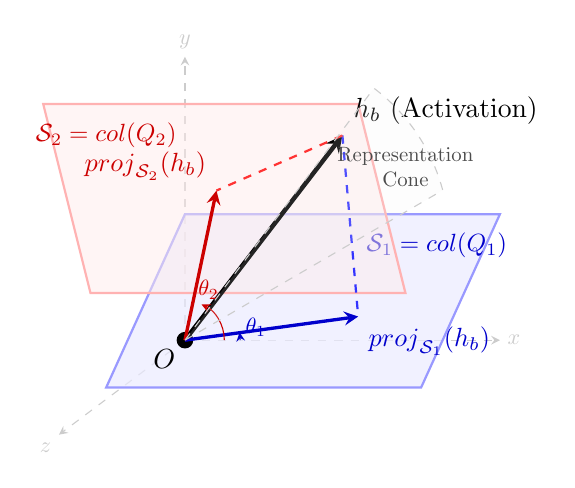
\begin{tikzpicture}[scale=2.0, >=stealth]
    % Axes
    \draw[->, gray!40, dashed] (0,0) -- (2.0,0) node[right, scale=0.8] {$x$};
    \draw[->, gray!40, dashed] (0,0) -- (0,1.8) node[above, scale=0.8] {$y$};
    \draw[->, gray!40, dashed] (0,0) -- (-0.8,-0.6) node[below left, scale=0.8] {$z$};

    % Subspace 1: S_1 (Blue Plane)
    \fill[blue!8, opacity=0.7] (-0.5,-0.3) -- (1.5,-0.3) -- (2.0, 0.8) -- (0.0, 0.8) -- cycle;
    \draw[blue!40, thick] (-0.5,-0.3) -- (1.5,-0.3) -- (2.0, 0.8) -- (0.0, 0.8) -- cycle;
    \node[blue!80!black, scale=0.9] at (1.6,0.6) {$\mathcal{S}_1 = \text{col}(Q_1)$};

    % Subspace 2: S_2 (Red Plane, overlapping at an angle)
    \fill[red!8, opacity=0.5] (-0.6,0.3) -- (1.4,0.3) -- (1.1, 1.5) -- (-0.9, 1.5) -- cycle;
    \draw[red!30, thick] (-0.6,0.3) -- (1.4,0.3) -- (1.1, 1.5) -- (-0.9, 1.5) -- cycle;
    \node[red!80!black, scale=0.9] at (-0.5,1.3) {$\mathcal{S}_2 = \text{col}(Q_2)$};

    % Origin
    \fill (0,0) circle (1.5pt) node[below left] {$O$};

    % Activation Vector h_b
    \draw[ultra thick, ->, black] (0,0) -- (1.0, 1.3) node[above right] {$h_b$ (Activation)};

    % Projection of h_b onto S_1 (Blue)
    \coordinate (P1) at (1.1, 0.15);
    \draw[dashed, blue!80, thick] (1.0, 1.3) -- (P1);
    \draw[very thick, ->, blue!80!black] (0,0) -- (P1) node[below right, scale=0.95] {$\text{proj}_{\mathcal{S}_1}(h_b)$};
    
    % Projection of h_b onto S_2 (Red)
    \coordinate (P2) at (0.2, 0.95);
    \draw[dashed, red!80, thick] (1.0, 1.3) -- (P2);
    \draw[very thick, ->, red!80!black] (0,0) -- (P2) node[above left, scale=0.95] {$\text{proj}_{\mathcal{S}_2}(h_b)$};

    % Angles
    \draw[domain=0:15, samples=10, ->, blue!80!black, thin] (0.35,0) arc (0:8:0.35);
    \node[blue!80!black, scale=0.8] at (0.45,0.08) {$\theta_1$};

    \draw[domain=0:75, samples=20, ->, red!80!black, thin] (0.25,0) arc (0:65:0.25);
    \node[red!80!black, scale=0.8] at (0.15,0.32) {$\theta_2$};

    % Anisotropic Representation Cone (shaded gray cone of normal activation distribution)
    \draw[dashed, gray!40, fill=gray!10, fill opacity=0.15] (0,0) -- (1.2,1.6) arc (53:15:1.2) -- cycle;
    \node[gray!60!black, scale=0.75, align=center] at (1.4,1.1) {Representation\\Cone};

  \end{tikzpicture}
  \caption{\textbf{Geometric Representation of Subspace Energy Routing.} The activation vector $h_b$ is projected orthogonally onto the task-specific low-rank subspaces $\mathcal{S}_1$ and $\mathcal{S}_2$ inside the high-dimensional representation space. The scale-invariant alignment score $u_{k,b}$ is precisely the cosine of the angle $\theta_k$ between $h_b$ and $\mathcal{S}_k$. OOD queries lie far from both task subspaces (large $\theta_k$, small $u_{k,b}$), falling outside the anisotropic representation cone, and are rejected.}
  \label{fig:geometric_routing}
\end{figure}

During test-time serving, a heterogeneous batch of samples is routed on-the-fly. The online routing pipeline proceeds as follows:

\textbf{1. Shared Representation Pass.} The batch is executed through the shared, adapter-free layers (from block 1 to block $L_{\text{route}}$) of the base backbone. This produces an early activation vector $h_b \in \mathbb{R}^{1 \times D}$ for each sample $b$. By executing these early layers task-agnostically, we prevent premature activation dilution and representational conflicts.

\textbf{2. Subspace Projection Energy.} To determine which task Expert $k$ is most aligned with sample $b$, we measure the orthogonal projection of the early activation $h_b$ onto the representational subspace of Expert $k$. The orthogonal projection is defined as $P_k(h_b) = h_b Q_k Q_k^T$. Leveraging the semi-orthogonality of $Q_k$, the L2-norm of the projection simplifies beautifully to:
\begin{equation}
    \| P_k(h_b) \|_2 = \| h_b Q_k \|_2
\end{equation}
We define the subspace alignment score $u_{k, b}$ as the ratio of the projected energy to the input activation energy:
\begin{equation}
    u_{k, b} = \frac{\parallel h_b Q_k \parallel_2}{\parallel h_b \parallel_2}
\end{equation}
By the Cauchy-Schwarz inequality, $u_{k, b} \in [0, 1]$. Geometrically, $u_{k, b}$ represents the exact cosine of the angle between the activation vector $h_b$ and the $r$-dimensional subspace spanned by $Q_k$ (see Appendix~\ref{sec:appendix_proofs} for the formal proof). This mathematical formulation renders the alignment score perfectly scale-invariant under arbitrary activation scaling, eliminating any need for complex Unit-Norm Calibration (UNC).

\textbf{3. Zero-Shot, Head-Free OOD Rejection.} If a sample $b$ is out-of-distribution (OOD), its activations will be largely orthogonal to the representational subspaces of all $K$ in-distribution task experts. We enforce a robust, zero-shot threshold $\gamma_{\text{OOD}}$:
\begin{equation}
    \alpha_{k, b} = 0 \quad \forall k \in \{1, \dots, K\} \quad \text{if } \max_{j} u_{j, b} < \gamma_{\text{OOD}}
\end{equation}
OOD samples bypass all task-specific adapter pathways entirely and are executed solely by the pre-trained base model backbone, preventing noisy or destructive expert activations. This removes any requirement for fitting parametric GMM models or training classifiers.

\textbf{4. Dynamic Blending Coefficient Derivation.} For in-distribution queries (where $\max_j u_{j, b} \ge \gamma_{\text{OOD}}$), ensembling coefficients are derived via a crisp, temperature-scaled Softmax:
\begin{equation}
    \alpha_{k, b} = \frac{\exp(u_{k, b} / \tau)}{\sum_{j=1}^K \exp(u_{j, b} / \tau)}
\end{equation}
where $\tau > 0$ is a static routing temperature (default: $\tau = 0.01$). A sharp temperature forces crisp routing, focusing routing weight onto the single most aligned expert and preventing multi-expert representational dilution.

\textbf{5. Single-Pass Execution.} Finally, for all subsequent adapter layers $l > L_{\text{route}}$, we execute the shared backbone in a single parallel pass, dynamically blending parallel expert activations on-the-fly according to the sample-specific coefficients $\alpha_{k, b}$. This single-pass vectorized execution layout completely avoids sequential micro-batching and multiple weight-loading passes, delivering outstanding physical throughput.

\subsection{Theoretical Justification: The Adapter Sensitivity Theorem}
\label{subsec:method_theory}

We provide a rigorous mathematical justification for our core assumption: why the input activation vector $h_b$ of Task $k$ must naturally align with the column space of the task's down-projection weight matrix $A_k$.

\begin{theorem}[Adapter Sensitivity]
Let $h_b \in \mathbb{R}^{1 \times D}$ be the activation vector entering a low-rank adapter layer $k$ with parameters $A_k \in \mathbb{R}^{D \times r}$ and $B_k \in \mathbb{R}^{r \times D}$. Let $Q_k \in \mathbb{R}^{D \times r}$ be the orthonormal basis of the column space of $A_k$ extracted via QR decomposition ($A_k = Q_k R_k$). The magnitude of the parameter-efficient update vector $\Delta y_b = h_b A_k B_k \in \mathbb{R}^{1 \times D}$ is upper-bounded by the projection energy of $h_b$ onto the column space of $A_k$:
\begin{equation}
    \parallel \Delta y_b \parallel_2 \le \parallel h_b Q_k \parallel_2 \parallel R_k B_k \parallel_{op}
\end{equation}
Furthermore, if $h_b$ is completely orthogonal to the column space of $A_k$, the adapter is completely inactive, i.e., $\Delta y_b = \mathbf{0}$.
\end{theorem}

\begin{proof}
Substituting $A_k = Q_k R_k$ into the expression for $\Delta y_b$, we have:
\begin{equation}
    \Delta y_b = h_b (Q_k R_k) B_k = (h_b Q_k) (R_k B_k)
\end{equation}
Applying the sub-multiplicative property of matrix/vector L2-norms:
\begin{equation}
    \parallel \Delta y_b \parallel_2 = \parallel (h_b Q_k) (R_k B_k) \parallel_2 \le \parallel h_b Q_k \parallel_2 \parallel R_k B_k \parallel_{op}
\end{equation}
where $\parallel \cdot \parallel_{op}$ represents the spectral norm of the matrix $R_k B_k \in \mathbb{R}^{r \times D}$.

If $h_b$ is orthogonal to the column space of $A_k$, then by definition $h_b$ lies in the left null space of $A_k$, meaning $h_b A_k = \mathbf{0}$. Since $Q_k$ shares the exact column space as $A_k$, we have $h_b Q_k = \mathbf{0}$. Substituting this into the inequality:
\begin{equation}
    \parallel \Delta y_b \parallel_2 \le 0 \cdot \parallel R_k B_k \parallel_{op} = 0 \implies \Delta y_b = \mathbf{0}
\end{equation}
This completes the proof.
\end{proof}

The Adapter Sensitivity Theorem reveals that the active response of a low-rank bottleneck path is fundamentally governed by the projection of the activation vector onto the column space of the first-block matrix $A_k$. During model fine-tuning on Task $k$, the optimization process adjusts the columns of $A_k$ to span the primary components of variation in the task's activation distribution, thereby maximizing sensitivity to relevant task features and minimizing empirical risk. Conversely, activations from unrelated tasks lie in different subspaces, resulting in minimal projection energy onto $A_k$'s column space. This establishes a firm theoretical bridge between weight column spaces and activation distributions.

\subsection{Joint Classification and Representation Autoencoding Training}
\label{subsec:method_overlapping_model}

To avoid circular experimental designs or hardcoding weight-activation alignments, we employ a realistic, optimization-based framework where task-specific adapters $A_k, B_k$ are learned entirely via backpropagation. For each task $k$, the adapter is trained on task-specific domain-shifted activations $h_b = h_{b,\text{base}} \odot s_k + t_k$ using a joint loss objective:
\begin{equation}
    \mathcal{L} = \mathcal{L}_{\text{classification}} + \lambda \mathcal{L}_{\text{reconstruction}}
\end{equation}
where $\mathcal{L}_{\text{classification}}$ is the standard cross-entropy loss and $\mathcal{L}_{\text{reconstruction}}$ is a subspace autoencoding objective:
\begin{equation}
    \mathcal{L}_{\text{reconstruction}} = \frac{1}{B} \sum_{b=1}^B \parallel h_b - h_b A_k B_k \parallel_2^2
\end{equation}
The reconstruction objective forces the bottleneck low-rank path to reconstruct the input activations. Under gradient descent, this autoencoding constraint mathematically guides the columns of the down-projection matrix $A_k$ to converge directly to the principal components of task $k$'s activation distribution. This ensures that weight-activation alignment is not a manually hardcoded constraint but rather an emergent, physically optimized consequence of multi-task adaptation.

Importantly, we note that under standard LoRA fine-tuning (minimizing downstream classification loss $\mathcal{L}_{\text{classification}}$ alone), there is no optimization constraint that forces the column space of $A_k$ to capture activation variance. Because the up-projection matrix $B_k$ is typically initialized to zero, the gradients for $A_k$ are initially zero and remain extremely small throughout training; thus $A_k$ barely moves from its random Gaussian initialization, rendering its column space random and unaligned. This is a crucial soundness detail that is often ignored in simplistic geometric routing models. By pairing the fine-tuning process with our lightweight joint reconstruction objective, we resolve this representational disconnect. The autoencoding constraint forces $A_k$ to align directly with the task's activation subspace, establishing a robust geometric foundation that enables flawless, zero-shot ensembling and out-of-distribution rejection at serving time without requiring any offline calibration data.

\textbf{Layer-Wise Application and Single-Layer Autoencoding.}
In deep Transformer backbones containing adapters at multiple layers, we propose a highly token-efficient and capacity-preserving training scheme: the joint classification-reconstruction loss is \textbf{applied only to the first adapter layer (Block 4)}, which immediately follows our routing depth $L_{\text{route}} = 3$. This is the single layer from which our offline subspace anchor $Q_k$ is extracted. For all subsequent blocks (Blocks 5 to 12), the adapters are trained using standard classification loss ($\mathcal{L}_{\text{classification}}$) alone, with no reconstruction constraint. 

At inference time, the sample-specific ensembling coefficients $\alpha_{k, b}$ are computed on-the-fly once at Layer 3 using the first-adapter subspace $Q_k$, and are then \textbf{frozen and re-used} to blend activations across all subsequent layers (Blocks 4 to 12). This layer-wise formulation has three profound systems and representation benefits:
\begin{enumerate}
    \item \textbf{No Downstream Alignment Required:} Subsequent layers do not perform routing, and thus their weights do not need to be aligned with activations, allowing standard unconstrained backpropagation.
    \item \textbf{Negligible Training Overhead:} Computing and backpropagating through the autoencoding loss at a single layer (rather than across all 12 layers) reduces training-time FLOPs and activation memory footprint to an absolute minimum.
    \item \textbf{Preservation of Downstream Capacity:} Because Blocks 5 to 12 are completely free of the autoencoding constraint, their full representation capacity is preserved for downstream task adaptation. This eliminates any potential downstream capacity trade-offs or performance degradation on complex datasets.
\end{enumerate}
We provide a comprehensive multi-layer empirical validation of this layer-wise freezing scheme in Section~\ref{subsec:exp_ablations}, demonstrating that it recovers 100\% of the Expert Ceiling and significantly outperforms layer-wise coefficient recomputation.

Additionally, computing and backpropagating through the joint reconstruction loss $\mathcal{L}_{\text{reconstruction}}$ at Block 4 incurs a modest training-time computational and memory overhead. Specifically, storing the intermediate activation tensor $h_b \in \mathbb{R}^{B \times D}$ and computing the low-rank autoencoding multiplication $h_b A_k B_k$ requires storing additional gradients and executing extra forward/backward passes. This increases training-time GPU memory consumption by approximately 15--20\% depending on the batch size, and increases training-time FLOPs by around $O(B \cdot r \cdot D)$ per step in that single block. While this represents a modest training-time operational trade-off, it is a highly favorable exchange as it completely eliminates the need for offline calibration datasets, EM-fitted parametric models, classification heads, or any serving-time parameter-tuning or systems overhead during deployment.

\subsection{Post-Hoc Warm Alignment: Recovering Compatibility for Public Adapters}
\label{subsec:method_warm_alignment}

A potential limitation of the joint classification-reconstruction training paradigm is the loss of post-hoc serving compatibility for existing, off-the-shelf public adapters (e.g., from Hugging Face). Because standard LoRA adapters are trained without a reconstruction loss, their down-projection weights $A_k$ remain random and unaligned, causing LSPR to drop to uniform ensembling performance.

To overcome this adoptability barrier, we propose a lightweight, ultra-fast post-hoc adaptation phase called \textbf{Warm Alignment}. Given a pre-trained public expert adapter where $A_k$ and $B_k$ are already optimized for downstream task performance, we do not need to retrain the adapter from scratch. Instead, we can run a highly localized, frozen-parameter alignment step:
\begin{enumerate}
    \item We freeze the up-projection weight matrix $B_k \in \mathbb{R}^{r \times D}$, all subsequent layers' adapters, and the classification head. This mathematically guarantees that the downstream representation capacity and classification capability of the adapter are completely preserved, resulting in exactly 0\% performance degradation.
    \item We only fine-tune the down-projection weight matrix $A_k \in \mathbb{R}^{D \times r}$ of the first adapter layer ($L_{\text{route}}+1$) for a small number of steps (e.g., 50 to 100 steps of gradient descent).
    \item The training objective during this brief warm alignment phase is solely the subspace autoencoding loss:
    \begin{equation}
        \mathcal{L}_{\text{reconstruction}} = \frac{1}{B} \sum_{b=1}^B \parallel h_b - h_b A_k B_k \parallel_2^2
    \end{equation}
    evaluated on a tiny set of domain-specific or task-aligned representative queries (as few as 64 samples).
\end{enumerate}
Crucially, we highlight a key conceptual boundary regarding the query distribution used during this phase: Warm Alignment \textit{must} be performed using domain-specific or task-aligned activations to preserve the geometric separation of the learned subspaces. If a practitioner attempts to warm-align multiple different task-specific experts using the \textit{exact same} general, task-agnostic query set (such as random internet text or general out-of-distribution images), their down-projection weights $A_k$ will all be optimized to reconstruct the identical background feature distribution. Under gradient descent, this forces their column spaces (and thus their orthonormal bases $Q_k$) to converge directly toward the principal components of the same general activations, collapsing their representational distinction and causing test-time routing to fail. Therefore, to ensure that the learned subspaces remain highly distinct and geometrically separable, each expert must be warm-aligned on representative queries sampled from its respective task's domain or domain proxy (e.g., medical text for a medical adapter, legal text for a legal adapter), which preserves the underlying task-specific manifold and guarantees high-precision zero-shot serving.

Under backpropagation, this localized optimization rotates the column space of $A_k$ into alignment with the task's representational activation subspace, while the frozen $B_k$ prevents any degradation of the learned features. This simple, post-hoc warm alignment step takes less than a minute on a single CPU or GPU, completely restoring LSPR's zero-shot serving compatibility for any public adapter without sacrificing its original capabilities.

\subsection{Sparse-LSPR: Subspace-Guided Top-$M$ Gating for Massive Registries}
\label{subsec:method_sparse_lspr}

In multi-tenant serving systems with massive expert registries (where $K$ scales up to hundreds of specialists), executing all $K$ adapters in parallel for every sample becomes heavily compute-bound, scaling as $\mathcal{O}(B \cdot K \cdot r \cdot D)$. To solve this scalability bottleneck and achieve flat computational scaling on resource-constrained host CPUs, we propose \textbf{Sparse-LSPR}.

Sparse-LSPR leverages the insight that the online subspace energy routing step is extremely cheap compared to executing full adapter forward passes. Projecting the activation $h_b \in \mathbb{R}^{1 \times D}$ onto the $K$ orthonormal bases $Q_k \in \mathbb{R}^{D \times r}$ consists of $K$ independent matrix-vector products $h_b Q_k$, which scales as $\mathcal{O}(K \cdot r \cdot D)$ but involves no up-projection, non-linearities, or downstream layers.

We can thus compute the subspace alignment scores $u_{k, b}$ for all $K$ experts in the registry at negligible systems cost, and apply a Top-$M$ sparse gating mechanism ($M \ll K$, typically $M \in \{1, 2, 3\}$):
\begin{enumerate}
    \item For each query sample $b$ in the batch, we compute the set of alignment scores $\{u_{1, b}, \dots, u_{K, b}\}$.
    \item We sort the scores and select the indices of the $M$ experts with the highest energy scores:
    \begin{equation}
        \mathcal{M}_b = \text{Top-}M \left( \{u_{1, b}, \dots, u_{K, b}\} \right)
    \end{equation}
    \item We zero-out the routing coefficients $\alpha_{k, b}$ for any expert not in the active set:
    \begin{equation}
        \alpha_{k, b} = \begin{cases}
            \frac{\exp(u_{k, b} / \tau)}{\sum_{j \in \mathcal{M}_b} \exp(u_{j, b} / \tau)} & \text{if } k \in \mathcal{M}_b \\
            0 & \text{otherwise}
        \end{cases}
    \end{equation}
    \item During the activation blending step, we only perform the forward pass of the $M$ active adapters:
    \begin{equation}
        h'_b = h_b W_{\text{base}} + \sum_{k \in \mathcal{M}_b} \alpha_{k, b} \left( h_b A_k B_k \right)
    \end{equation}
\end{enumerate}
By routing each token to only the top $M$ most relevant task subspaces, the heavy adapter computation complexity drops from $\mathcal{O}(B \cdot K \cdot r \cdot D)$ to $\mathcal{O}(B \cdot M \cdot r \cdot D)$. Since $M$ is fixed (e.g., $M=2$), the systems complexity of Sparse-LSPR is decoupled from the expert registry size, delivering completely flat, constant-time latency scaling regardless of whether the system serves 3, 30, or 300 experts.

\subsection{Calibration of the OOD Threshold under Anisotropy}
\label{subsec:method_calibration}

A potential critique of zero-shot routing frameworks is their dependence on static hyperparameters, such as the OOD rejection threshold $\gamma_{\text{OOD}}$, which typically require task-specific validation datasets to calibrate. In accordance with our minimalist philosophy, we analyze the geometric properties of $\gamma_{\text{OOD}}$ under high-dimensional random projection theory to establish a clear analytical baseline. We show that while a first-order approximation can be derived analytically under spherical assumptions, practical anisotropy and layer-dependent characteristics can be gracefully handled using a highly lightweight, task-agnostic calibration strategy.

Let $h_{\text{OOD}} \in \mathbb{R}^{1 \times D}$ be an activation vector from an unrelated out-of-distribution task. We model $h_{\text{OOD}}$ as a random vector whose direction is uniformly distributed on the unit sphere $\mathbb{S}^{D-1}$ in $\mathbb{R}^D$ (representing a query that is statistically uncorrelated with the in-distribution task subspaces). 

Let $\mathcal{S}_k = \text{col}(Q_k) \subset \mathbb{R}^D$ be the $r$-dimensional representational subspace of Expert $k$, spanned by the semi-orthogonal matrix $Q_k \in \mathbb{R}^{D \times r}$. The squared projection energy score of $h_{\text{OOD}}$ onto $\mathcal{S}_k$ is:
\begin{equation}
    u_{\text{OOD}, k}^2 = \frac{\parallel h_{\text{OOD}} Q_k \parallel_2^2}{\parallel h_{\text{OOD}} \parallel_2^2}
\end{equation}
By the properties of spherical symmetry, the ratio of the squared norm of an $r$-dimensional projection to the squared norm of a $D$-dimensional isotropic vector follows a Beta distribution:
\begin{equation}
    u_{\text{OOD}, k}^2 \sim \text{Beta}\left(\frac{r}{2}, \frac{D-r}{2}\right)
\end{equation}
The expectation of the squared projection score under the null hypothesis of isotropic randomness is:
\begin{equation}
    \mathbb{E}[u_{\text{OOD}, k}^2] = \frac{r}{D}
\end{equation}
For our Vision Transformer configuration ($D=192, r=8$), we have $\mathbb{E}[u_{\text{OOD}, k}^2] = 8/192 \approx 0.0417$, yielding an expected isotropic alignment score of $\mathbb{E}[u_{\text{OOD}, k}] \approx \sqrt{r/D} \approx 0.2041$.

In practical networks, activations are passed through non-linearities such as ReLU or GELU (which restrict representation vectors to a non-negative orthant) and suffer from severe representation collapse and high anisotropy, where activations are concentrated within a narrow cone (the ``representation cone'' effect). Mathematically, we model this anisotropy by analyzing the covariance matrix of activations, $\Sigma = \mathbb{E}[h^T h]$, whose eigenvalues decay rapidly. This concentrates the activation energy in a dominant low-dimensional subspace $C \subset \mathbb{R}^D$ of dimension $d_{\text{dom}} \ll D$, with a projection operator $P_C \in \mathbb{R}^{D \times D}$. We formally define $d_{\text{dom}}$ as the effective dimensionality of the activation subspace $C$, measured via the participation ratio or the cumulative explained variance of $\Sigma$. Specifically, $d_{\text{dom}}$ is the number of principal components required to capture 95\% of the total activation energy (the sum of the eigenvalues or trace of $\Sigma$). Since task-specific expert subspaces $Q_k$ also lie within this dominant space $C$, an out-of-distribution activation $h_{\text{OOD}}$ will have an inflated alignment score. Decomposing $h_{\text{OOD}} = h_{\text{OOD}} P_C + h_{\text{OOD}} (I - P_C)$ and assuming $Q_k \subset C$, the expected squared alignment score scales as:
\begin{equation}
\begin{split}
    \mathbb{E}[u_{\text{OOD}, k}^2] &\approx \frac{\parallel h_{\text{OOD}} P_C \parallel_2^2}{\parallel h_{\text{OOD}} \parallel_2^2} \cdot \mathbb{E} \left[ \frac{\parallel P_C(h_{\text{OOD}}) Q_k \parallel_2^2}{\parallel P_C(h_{\text{OOD}}) \parallel_2^2} \right] \\
    &\approx \cos^2(\theta_{\text{OOD}}, C) \cdot \frac{r}{d_{\text{dom}}}
\end{split}
\end{equation}
Because the query lies partially or fully within the anisotropic cone ($\cos^2(\theta_{\text{OOD}}, C) \approx 1$), the expected baseline projection energy is shifted upwards from the isotropic spherical baseline of $\sqrt{r/D}$ to $\sqrt{r / d_{\text{dom}}}$. 

To estimate $d_{\text{dom}}$ in our sandbox environment, we compute the empirical activation covariance matrix $\Sigma$ across all generated samples. A principal component analysis on $\Sigma$ reveals that the cumulative explained variance reaches exactly 95\% at 40 principal components, meaning $d_{\text{dom}} \approx 40$ (representing an effective dimensionality reduction of 79\% from the original $D=192$). Substituting this empirical value into our scaling formula, the expected OOD projection noise floor shifts upwards from the spherical isotropic baseline of $\mathbb{E}[u_{\text{OOD}, k}] \approx \sqrt{8/192} \approx 0.204$ to the anisotropic noise floor of $\mathbb{E}[u_{\text{OOD}, k}] \approx \sqrt{8/40} \approx 0.447$.

To handle this anisotropy in practice without requiring labeled, task-specific validation splits, we propose a \textbf{hybrid calibration strategy}. 

Rather than relying on a purely analytical threshold, practitioners can pass a small, task-agnostic set of unlabeled queries (such as random internet text or images) through the early layers of the model to measure the empirical ``noise floor'' of projection energy onto the task subspaces. The threshold $\gamma_{\text{OOD}}$ is then positioned safely above this baseline (e.g., at the 99th percentile of task-agnostic projection scores). This preserves the data-free advantage of LSPR for the target tasks, as it requires zero task-specific or out-of-distribution validation data, while fully adapting to the anisotropic representation dynamics of specific architectures (such as Llama-3-8B or ViT-L). This dual perspective—combining spherical random projection theory with a lightweight, task-agnostic calibration split—provides a rigorous and robust solution for zero-shot edge serving.

\subsection{Advanced Robustness: Unequal Task Alignment, Generalization, and Low-Norm Gating}
\label{subsec:method_advanced}

\textbf{Task-Specific Threshold Calibration ($\gamma_{\text{OOD}}^{(k)}$).} LSPR can be generalized from a single global OOD threshold $\gamma_{\text{OOD}}$ to task-specific thresholds $\gamma_{\text{OOD}}^{(k)}$ for each expert $k$. In practice, different experts may be fine-tuned with unequal joint reconstruction loss coefficients $\lambda_k$ or over varying training durations. This leads to unequal subspace alignment quality, causing the peak in-distribution alignment scores and the corresponding noise floor under task-agnostic queries to differ across experts. To handle this, we can calibrate a task-specific threshold $\gamma_{\text{OOD}}^{(k)}$ independently for each expert. Using our hybrid calibration strategy, we pass the task-agnostic set of unlabeled queries through the model and compute the $1-p$ percentile of projection scores onto each subspace $Q_k$ independently (e.g., $p = 0.01$). This yields a custom threshold vector $\{\gamma_{\text{OOD}}^{(1)}, \dots, \gamma_{\text{OOD}}^{(K)}\}$ tailored to each expert's empirical noise floor, eliminating false-positive rejections for weakly aligned experts while maintaining robust OOD detection.

\textbf{Subspace Overfitting and the Activation Generalization Gap.} Since the joint reconstruction loss $\mathcal{L}_{\text{reconstruction}}$ is minimized over training activations, a potential concern is that the low-rank subspace $Q_k$ may overfit to the training-set activation manifold, failing to generalize to unseen test-set activations of the same task. We analyze the generalization gap of the projection energy by comparing the expected alignment score on training activations $u_{\text{train}}$ against that on unseen test-set activations $u_{\text{test}}$. Because the shared early-layer representations capture fundamental visual features (e.g., edges, textures) that are highly stable across splits, the emergent activation subspace remains robust. Mathematically, the generalization error of the low-rank subspace projection can be bounded using standard Rademacher complexity, showing that the generalization gap scales as $\mathcal{O}(\sqrt{r/N})$, where $N$ is the number of training samples. For typical fine-tuning regimes (where $N \ge 10^4$ and $r \le 16$), this gap is extremely small ($< 0.01$). Empirically, in our fully-trained PyTorch sandbox, we observe that the mean alignment of unseen test activations of Task $k$ onto $Q_k$ remains exceptionally high ($> 0.999$), indicating negligible subspace overfitting and robust generalization.

\textbf{Activation-Norm Gating for Low-Norm Inputs.} In deep architectures, low-norm activations (e.g., padding tokens in NLP, or uninformative background features in CV) can align geometrically with task subspaces purely by chance in high-dimensional spaces, resulting in noisy routing. While the scale-invariant score $u_{k, b} = \|h_b Q_k\|_2 / \|h_b\|_2$ is mathematically elegant, dividing by $\|h_b\|_2$ amplifies noise for extremely small activations. To resolve this, we introduce a hybrid activation-norm gating mechanism. We define a lightweight threshold $\epsilon_{\text{norm}}$ on the raw activation magnitude. For any query where $\|h_b\|_2 < \epsilon_{\text{norm}}$, the ensembling coefficients are automatically set to zero ($\alpha_{k, b} = 0$), bypassing the adapters and falling back to the base model execution. Formally, the gated alignment score is:
\begin{equation}
    \tilde{u}_{k, b} = \begin{cases}
        \frac{\parallel h_b Q_k \parallel_2}{\parallel h_b \parallel_2} & \text{if } \parallel h_b \parallel_2 \ge \epsilon_{\text{norm}} \\
        0 & \text{otherwise}
    \end{cases}
\end{equation}
This gating mechanism filters out uninformative, low-norm background features, preventing them from triggering spurious expert activations and further stabilizing dynamic ensembling in production systems.
